\chapter{赋能企业结构变革}
\label{chapter:Enterprise}
习近平总书记强调科技创新在发展新质生产力中的核心地位,两会也着重提出推进 “人工智能 +” 行动。在此背景下,科技创新(人工智能)作用于教育所培养出的创新型人才,正从多方面深刻影响着企业结构。

\section{风险投资金额注入企业科技创新}
风险投资(Venture Capital,VC)是推动技术创新与经济增长的关键动力,其发展水平在一定程度上反映了国家在创新投入与政策支持上的力度。基于和鲸平台的《主要国家历年风险投资金额》,我们展示了2000至2023年中国、日本、法国和芬兰风险投资额的走势。图表分别采用原始值和对数尺度,直观反映各国风险投资发展的动态变化(见图\ref{fig:主要国家风险投资金额趋势})。

\begin{figure}[H]
    \centering
    % 左侧图
    \begin{subfigure}[b]{0.45\linewidth} % 调整宽度为画布宽度的45%
        \centering
        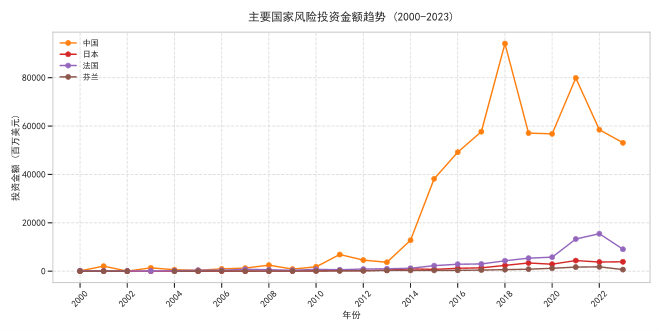
\includegraphics[width=\linewidth]{figure/07主要国家风险投资金额趋势.png}
        \caption{风险投资金额\_原始趋势}
        \label{fig:风险投资金额_原始趋势}
    \end{subfigure}
    \hfill % 增加子图之间的间距
    % 右侧图
    \begin{subfigure}[b]{0.45\linewidth}
        \centering
        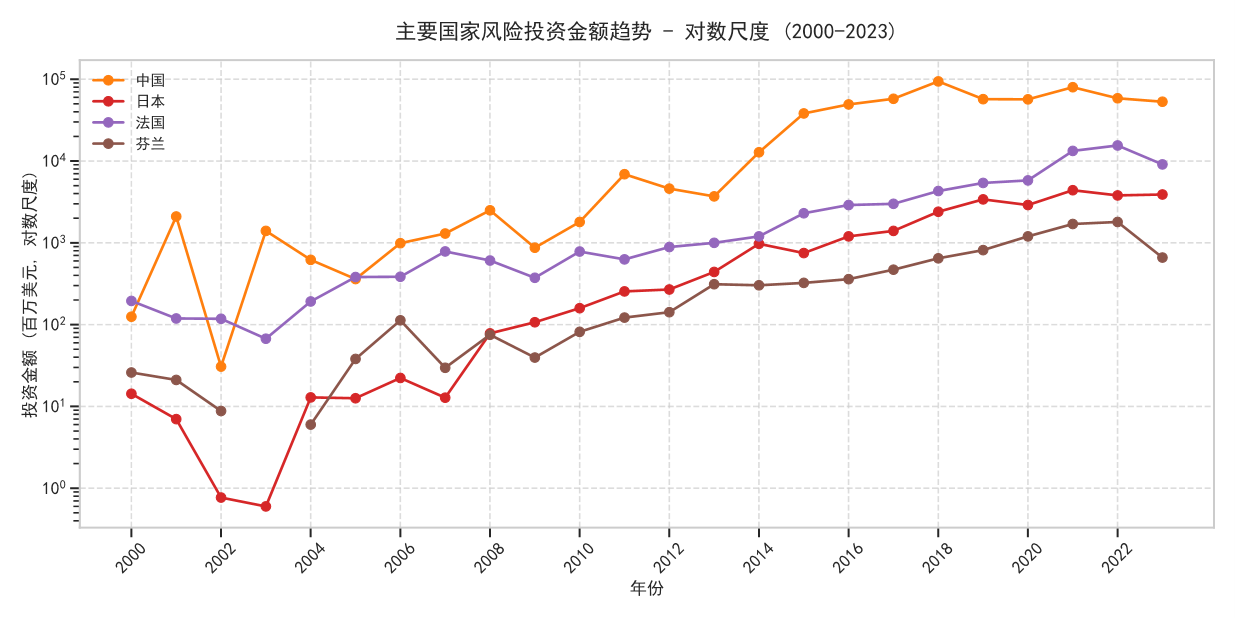
\includegraphics[width=\linewidth]{figure/06主要国家风险投资金额趋势-对数尺度.png}
        \caption{风险投资金额\_对数趋势}
        \label{fig:风险投资金额_对数趋势}
    \end{subfigure}
    \caption{风险投资金额原始趋势与对数趋势对比}
    \label{fig:主要国家风险投资金额趋势}
\end{figure}

中国在图\ref{fig:风险投资金额_原始趋势}中表现出显著的风险投资增长态势,尤其在2014至2018年期间,投资额几乎呈指数式上升,并在2018年达到近9万亿元的峰值\cite{Chen2022}。尽管自2019年后有所回落,总体投资水平依然居高不下。而图\ref{fig:风险投资金额_对数趋势}则从相对变化的角度展现了各国投资趋势,反映出各国在创新驱动经济发展中对资源配置和政策侧重点的不同。

中国的风险投资额在2014年至2018年经历了显著的快速增长,这一阶段得益于政策支持、资本市场开放以及新兴技术领域的迅速发展,从而奠定了中国在全球创新生态中的领先地位。这种大幅提升不仅彰显了中国在风险投资领域的崛起,也为未来发展提出了新的挑战,即如何在持续保持高投资额的同时,通过高效配置资源来最大化技术价值。

\section{独角兽公司发展趋势}
独角兽是指成立不到10年但估值10亿美元以上,又未在股票市场上市的科技创业公司。这些公司通常具有强大的创新能力和成长性,是新经济发展的风向标,也是新质生产力的典型代表。

\subsection{中国现存独角兽企业}
在中国现存独角兽企业部分,数量与估值的变化趋势不仅反映出创业生态环境的演变,也展示了资本市场对新兴行业的关注和投入。根据和鲸平台、睿兽分析的《主要国家独角兽公司数量》数据集,制作了“2013-2023年中国市场独角兽存续总数量变化”的柱状图和“2013-2023年中国存量独角兽平均估值变化”的折线图(见图\ref{fig:独角兽数量与估值变化})。

\begin{figure}[H]
    \centering
    % 左侧图
    \begin{subfigure}[b]{0.45\linewidth} % 调整宽度为画布宽度的45%
        \centering
        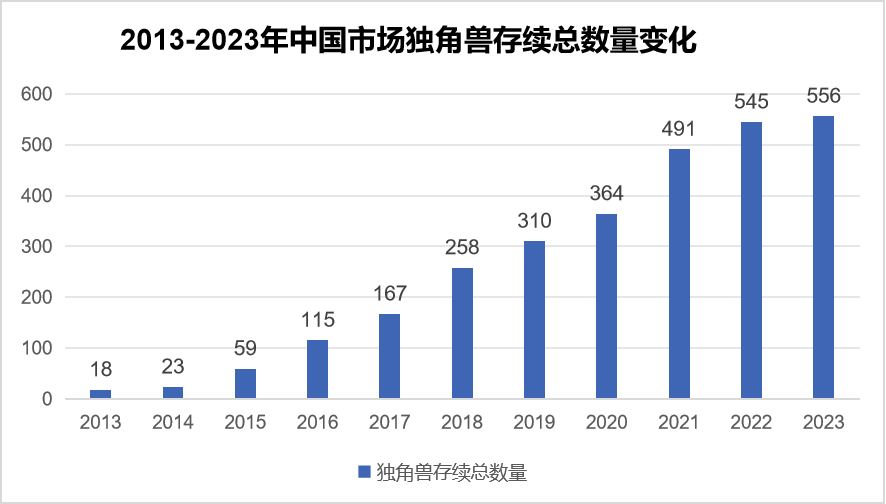
\includegraphics[width=\linewidth]{figure/08中国市场独角兽存续总数量变化.png}
        \caption{2013-2023年中国市场独角兽存续总数量变化}
        \label{fig:独角兽存续数量}
    \end{subfigure}
    \hfill % 增加子图之间的间距
    % 右侧图
    \begin{subfigure}[b]{0.45\linewidth}
        \centering
        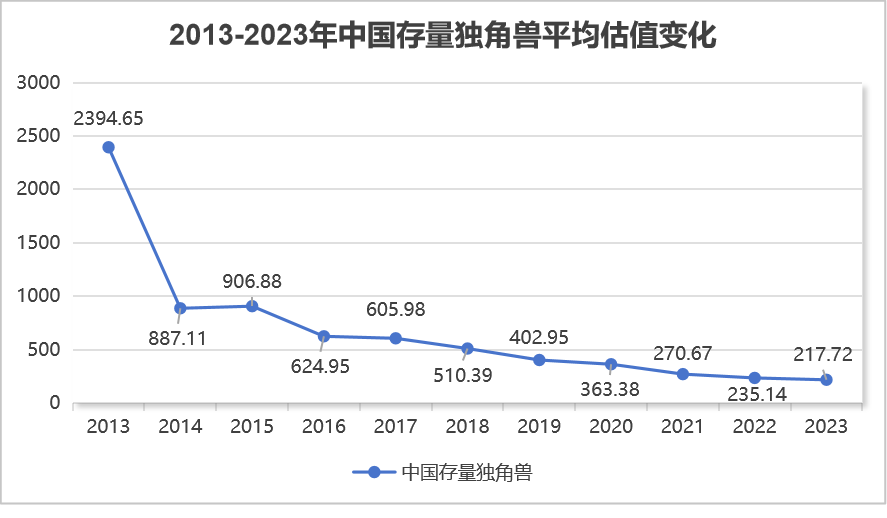
\includegraphics[width=\linewidth]{figure/09中国存量独角兽平均估值变化.png}
        \caption{2013-2023年中国存量独角兽平均估值变化}
        \label{fig:独角兽平均估值}
    \end{subfigure}
    \caption{中国市场独角兽的数量与估值变化趋势}
    \label{fig:独角兽数量与估值变化}
\end{figure}

从图\ref{fig:独角兽存续数量}可见,过去十年中国独角兽企业数量快速增长,尤其在2015至2021年间,从59家激增至491家,年均增幅明显,显示出政策支持、资本注入和技术创新共同推动了孵化能力的提升。但2022年和2023年的增速有所放缓,总量分别为545家和556家,可能与全球经济放缓及宏观环境不确定性有关。

同时,图\ref{fig:独角兽平均估值}显示,2013年至2023年间中国独角兽企业平均估值从2394.65亿元急剧下降至217.72亿元,降幅超过90\%。这可能是由于企业数量激增分散了头部优势,加之资本市场对企业盈利和可持续发展的重视,使估值标准趋于理性。

两组数据综合显示,企业数量的爆发性增长反映了创业生态活跃及资本支持力度强\cite{Xu2024},但增长放缓提示资源配置亟待优化,防止资本过度集中。其次,估值大幅下降表明市场正从“数量驱动”向“质量驱动”转变,更有利于培养具备长期竞争力的企业,同时也反映出资本对宏观经济和行业前景预期的变化。

总体来看,中国独角兽企业在近十年经历了数量激增与估值下调的现象,显示市场正从扩张向理性调整过渡。政策制定者和市场各方需更加注重支持高质量增长,通过优化资本配置、提升技术创新和推动企业可持续发展,确保企业在全球竞争中保持领先。同时,独角兽企业需从依赖高估值转变为注重核心技术和商业模式创新,以实现长期稳健发展。

\subsection{中国新晋独角兽企业}

近年来,中国现存独角兽企业数量的不断增长显示了创业生态的活跃性和资本市场的强力支持。在此基础上,深入分析新晋独角兽在各行业和重点省市的分布,有助于识别具备爆发潜力的领域和未来创新高地,从而为政策制定和资本布局提供参考。基于和鲸平台、睿兽数据集,制作了“2021-2013年中国新晋独角兽细分行业分布”的柱状图和“中国重点省市独角兽情况”的柱状折线图(见图\ref{fig:独角兽行业与区域分布}),以揭示新晋独角兽在行业和区域上的动态变化。

\begin{figure}[H]
    \centering
    % 左侧图
    \begin{subfigure}[b]{0.45\linewidth} % 调整宽度为画布宽度的45%
        \centering
        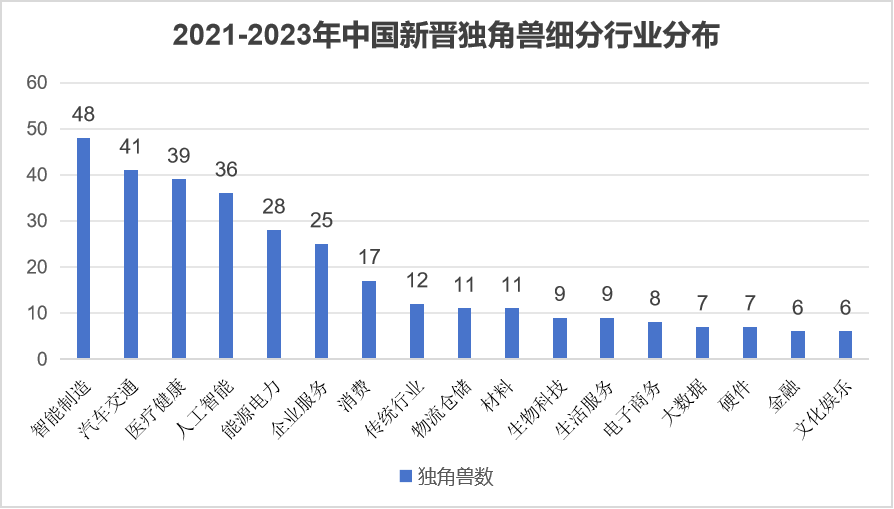
\includegraphics[width=\linewidth]{figure/10中国新晋独角兽细分行业分布.png}
        \caption{2021-2013年中国新晋独角兽细分行业分布}
        \label{fig:新晋独角兽行业分布}
    \end{subfigure}
    \hfill % 增加子图之间的间距
    % 右侧图
    \begin{subfigure}[b]{0.45\linewidth}
        \centering
        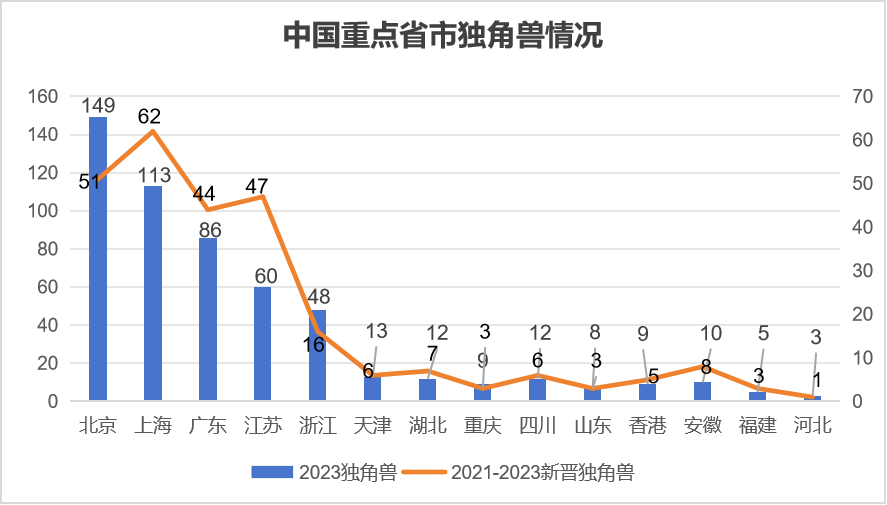
\includegraphics[width=\linewidth]{figure/11中国重点省市独角兽情况.png}
        \caption{中国重点省市独角兽情况}
        \label{fig:重点省市独角兽}
    \end{subfigure}
    \caption{中国新晋独角兽行业分布与重点省市情况对比}
    \label{fig:独角兽行业与区域分布}
\end{figure}

从图\ref{fig:新晋独角兽行业分布}中可以看出,智能制造、汽车交通和医疗健康是新增独角兽企业数量最多的三个行业,分别达到48家、41家和39家,处于主导地位。这表明,中国的独角兽企业正逐步向高端制造、生物医疗等技术密集型领域聚拢,反映出国家对战略性新兴产业的强力支持以及市场对高技术领域的投资热情。同时,人工智能、能源电力和企业服务等领域的新增独角兽数量也较为可观,进一步彰显了中国经济转型过程中对数字化、智能化和服务化发展的高度重视。

产业链与创新链的深度融合,正推动长三角地区成为中国近三年独角兽增长最快的区域。从区域分布看,独角兽企业往往集中在科研、人才、机构、企业优势明显的省市。图\ref{fig:重点省市独角兽}显示,截至2023年,北京、上海和广东分别拥有149家、113家和86家独角兽企业,遥遥领先;浙江和江苏也以60家和48家紧随其后。值得注意的是,2021年至2023年间,北京新增独角兽达51家,占全国新增比例显著,进一步巩固了其国家创新中心的地位;上海和广东分别新增62家和44家,强化了长三角和珠三角的引领作用。天津、湖北、四川等地虽然总量较少,但在新增数量上也展现出增长潜力。

未来,在确保核心区域依然保持领先优势的同时,如何进一步提升中西部及非一线城市的创新能力,将成为优化中国独角兽企业空间布局的关键。为此,建议政策制定者加大对欠发达地区创新生态的支持力度,同时持续推动高技术领域的研发投入与产业化进程,以助力中国独角兽企业迈向高质量发展。

\section{科技创新引领企业发展}
规模以上工业企业的研发活动被视为推动产业技术进步和实现经济高质量发展的关键力量。正因如此,本研究基于国家统计局和和鲸平台提供的《规模以上工业企业的科技活动基本情况》数据集,制作了“规模以上工业企业研发活动情况及预测”柱状折线图(见图\ref{规模以上工业企业研发活动情况及预测})。该图表利用融合模型预测了2004年至2030年期间企业参与研发活动的数量及其占比变化趋势,为评估工业企业未来研发投入及技术创新趋势提供了有力依据。

\begin{figure}[H]
    \centering
    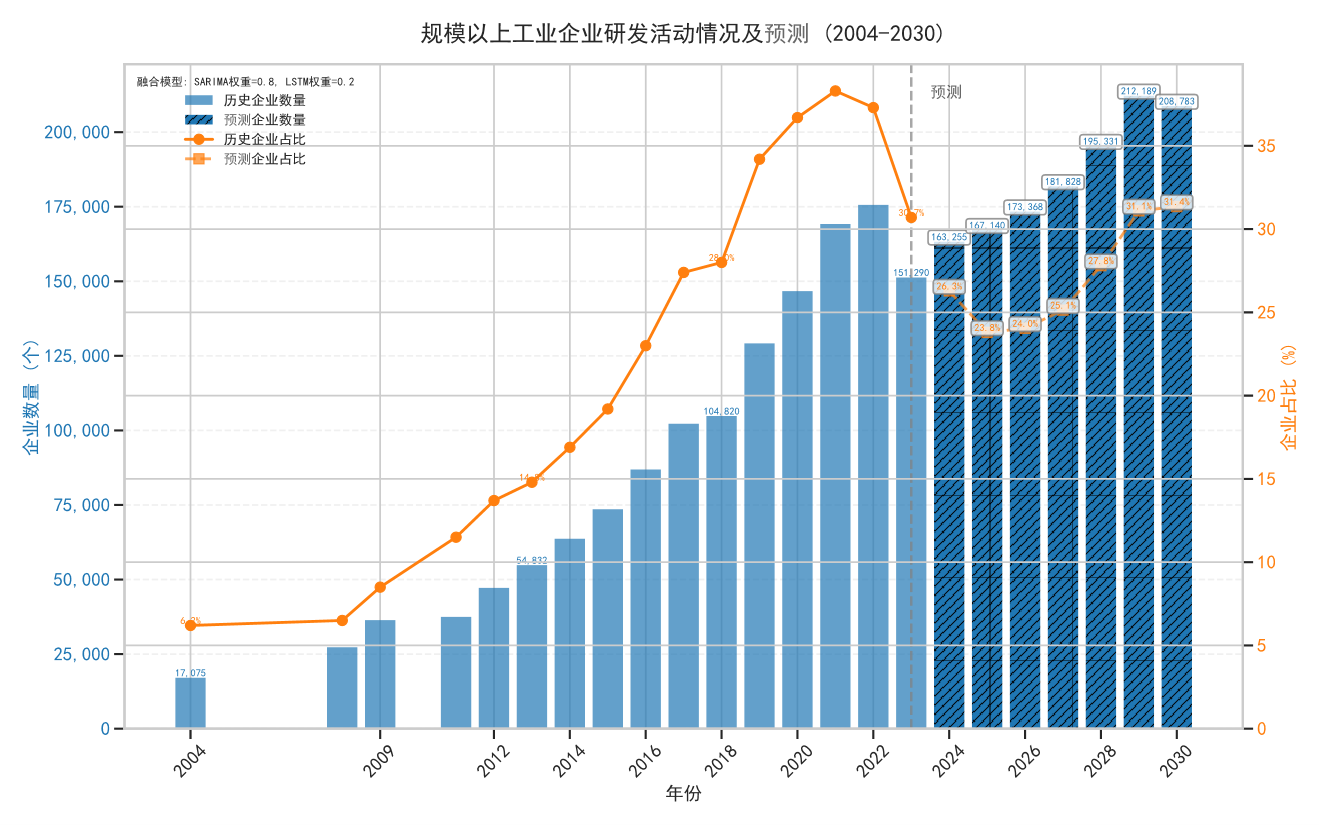
\includegraphics[width=0.7\linewidth]{figure/12规模以上工业企业研发活动情况及预测.png}
    \caption{规模以上工业企业研发活动情况及预测}
    \label{规模以上工业企业研发活动情况及预测}
\end{figure}


从2004年至2020年,规模以上工业企业参与研发活动的数量显著增长,从17,075家增加到151,290家,年均增长率较高。这显示出企业对技术创新的重视及政策对研发投入的激励作用\cite{WenZhao2021}。同时,研发活动占比由6\%上升至约30\%,表明研发已成工业企业发展的核心。值得注意的是,虽然2018年研发占比达到34\%的高点,但2020年后企业数量增速放缓,预计到2030年将达到212,189家,研发占比维持在31\%左右。这或许反映了市场成熟度、技术扩散和政策调整的影响,同时也说明了研发重心正由数量扩张转向质量提升。

未来,随着企业研发活动数量增速趋缓和占比稳定,重点应转向提升研发活动的质量与效率。建议进一步完善政策支持,鼓励高新技术企业加强基础研究与技术攻关,同时推动中小企业通过协同创新提升研发能力。此外,加强研发成果转化和应用,并完善知识产权保护机制,将有助于企业在全球竞争中保持技术优势。

\section{企业生产新产品促进市场}
随着人工智能技术的迅猛发展,其在社会生活、商业应用和产业创新中的影响不断增强。但公众对人工智能的认知与接受存在分歧,技术普及的同时也引发了隐私保护、伦理偏见和技术透明性等方面的担忧。在此背景下,人工智能的广泛应用引起了各界高度关注,尤其是生成式AI、自动化系统和智能服务的发展,既加速了技术落地,又带来了众多复杂的社会问题。基于和鲸平台的数据集,我们制作了“全球对人工智能产品与服务的看法(占比与总体百分比)——2022 VS 2023”柱状图(见图\ref{全球对人工智能产品与服务的看法(占比与总体百分比)——2022 VS 2023})。

\begin{figure}[H]
    \centering
    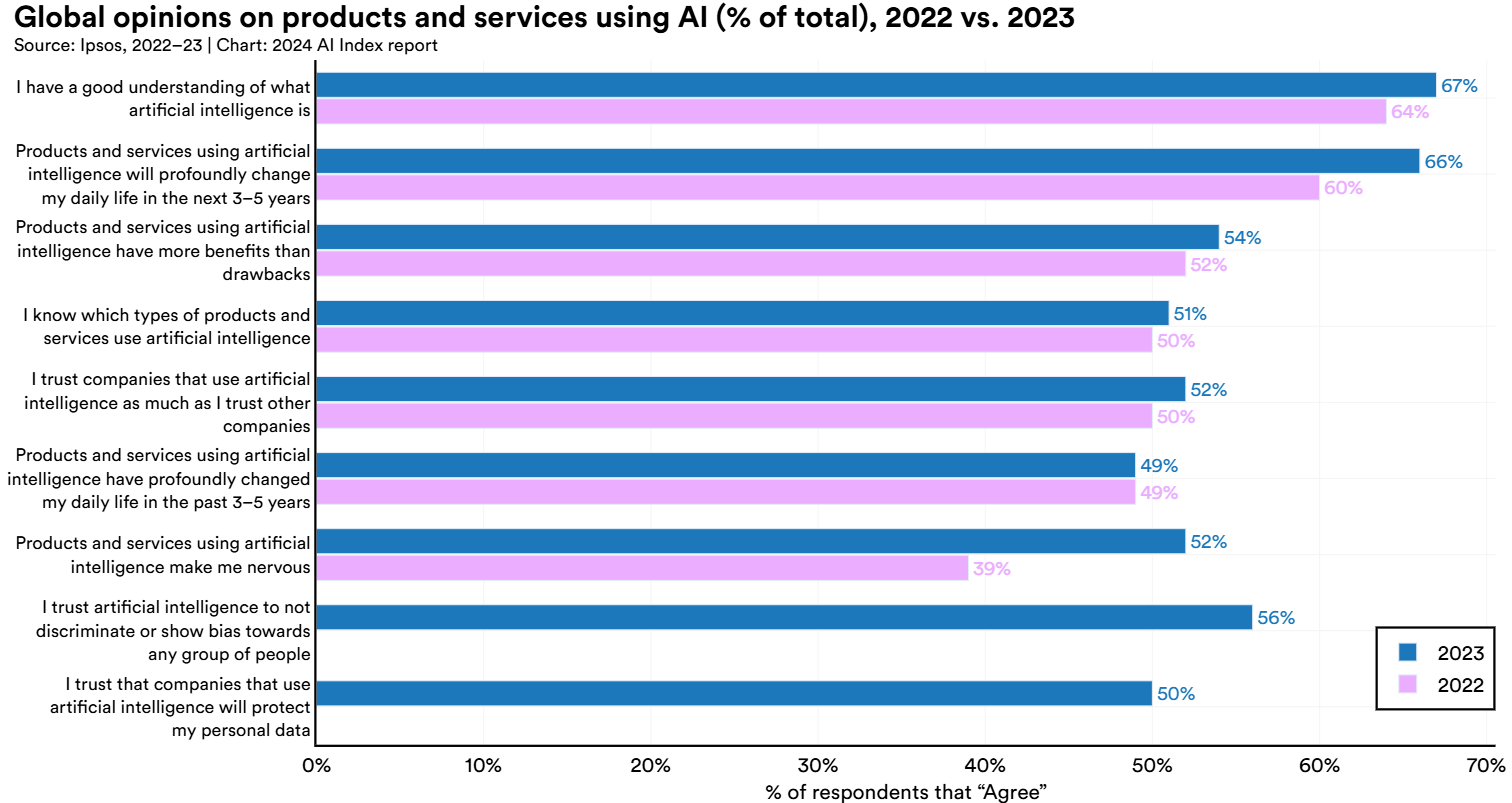
\includegraphics[width=0.7\linewidth]{figure/13全球对人工智能产品与服务的看法(占比与总体百分比)——2022 VS 2023.png}
    \caption{全球对人工智能产品与服务的看法(占比与总体百分比)——2022 VS 2023}
    \label{全球对人工智能产品与服务的看法(占比与总体百分比)——2022 VS 2023}
\end{figure}

数据显示,公众对AI的理解程度由64\%升至67\%,认为其将在未来3至5年深刻改变生活的比例由60\%增至66\%,而“好处多于缺点”的认同率由52\%小幅提升至54\%。与此同时,信任“使用AI的公司会保护个人数据”的比例维持在50\%,但感到紧张的比例却由39\%大幅上升到52\%,反映出对技术高速发展的不确定性;另外,有49\%的受访者认为AI在过去3至5年中对生活产生了深远影响,表明实际影响正在逐步累积。

综合来看,公众对人工智能的认知和接受度正在提高,体现了技术普及和广泛应用的趋势,而隐私保护和技术中立性方面的信任问题依然突出\cite{Zuiderwijk2021},伦理、偏见与监管风险引发的担忧也在增加。未来,技术提供者与政策制定者应致力于提升技术透明度、加强隐私保护和优化用户体验,同时通过科普和教育进一步普及AI知识,以构建更高的信任感,推动人工智能健康发展和广泛应用。

\section{风险投资金额注入企业科技创新}
为探讨未来社会变革对科技创新的反作用力,基于和鲸平台《主要国家历年风险投资金额》数据集,绘制了“中国风险投资金额历史数据与融合预测(2000-2030年)”折线图(如图\ref{中国风险投资金额历史数据与融合预测(2000-2030年)})。该图展示了2000年至2030年间中国风险投资金额的历史走势及融合模型的预测结果,为科学评估中国风险投资的长期发展趋势和制定相关政策提供了坚实的数据支持。

\begin{figure}[H]
    \centering
    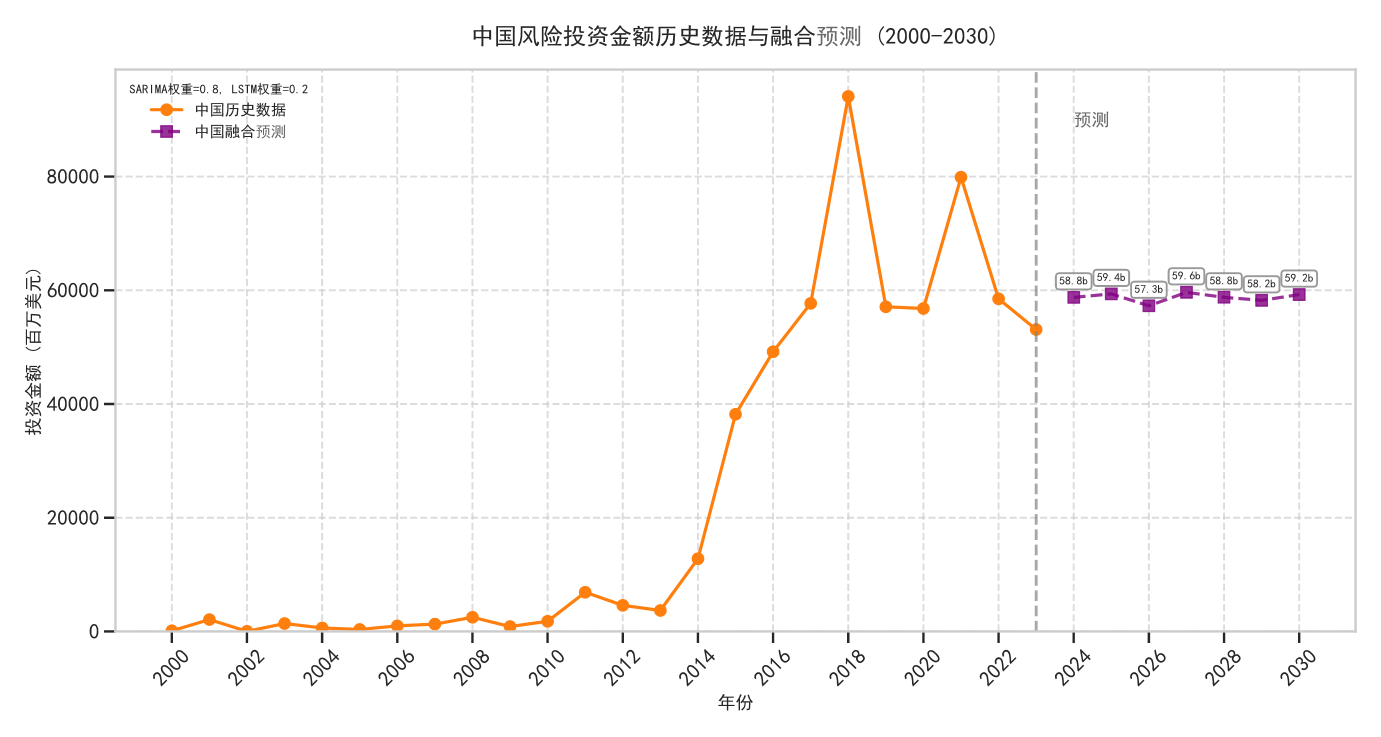
\includegraphics[width=0.7\linewidth]{figure/14中国风险投资金额历史数据与融合预测.png}
    \caption{中国风险投资金额历史数据与融合预测(2000-2030年)}
    \label{中国风险投资金额历史数据与融合预测(2000-2030年)}
\end{figure}

根据预测数据,2024年至2030年间,中国风险投资金额预计将趋于稳定,维持在约59,000百万美元左右。不过,受疫情以来市场剧烈波动的影响,该预测仍存在不确定性,可能需要结合更精确的经济学模型进行量化分析。

在未来,随着风险投资金额的稳定,投资重心将进一步转向高价值和高科技项目。为提升资本配置效率,建议政策制定者优化现有政策环境,鼓励多元化投资渠道的发展,并加大对新兴技术领域的支持力度。同时,风险投资机构应更加注重评估企业核心技术实力及长期发展潜力,推动创新生态系统的可持续发展。
